\newpage
\section{Concluding Remarks}
This work developed a uniquely identifiable parametric hybrid nonlinear model structure for SCR-ASC dynamics based on
the first principles. The RLS estimation results show the goodness of fit for the model. The parameters are not distinct
with respect to the aging of the catalyst. The parametric structure is unique while the actual parameter and regression
vectors can be tweaked based on models for rate constants, residence time and urea injection. This allows us to choose
appropriate assumptions for the reduced order model for the process. The uniqueness and the value of this method lies in
the explicit consideration of the effects of sampling on the system, and it's interplay with the residence time, while
having an identifiable model structure. Further analysis of the governing equations derived based on the molar
conservation, and it's interplay with sampling and residence time resulting in the emergence averaged effects needs to
be further analyzed to improve the prediction error for the parametric model.


\subsection{A review of the problems identified and solved}

\begin{figure}[H]
        \centering
        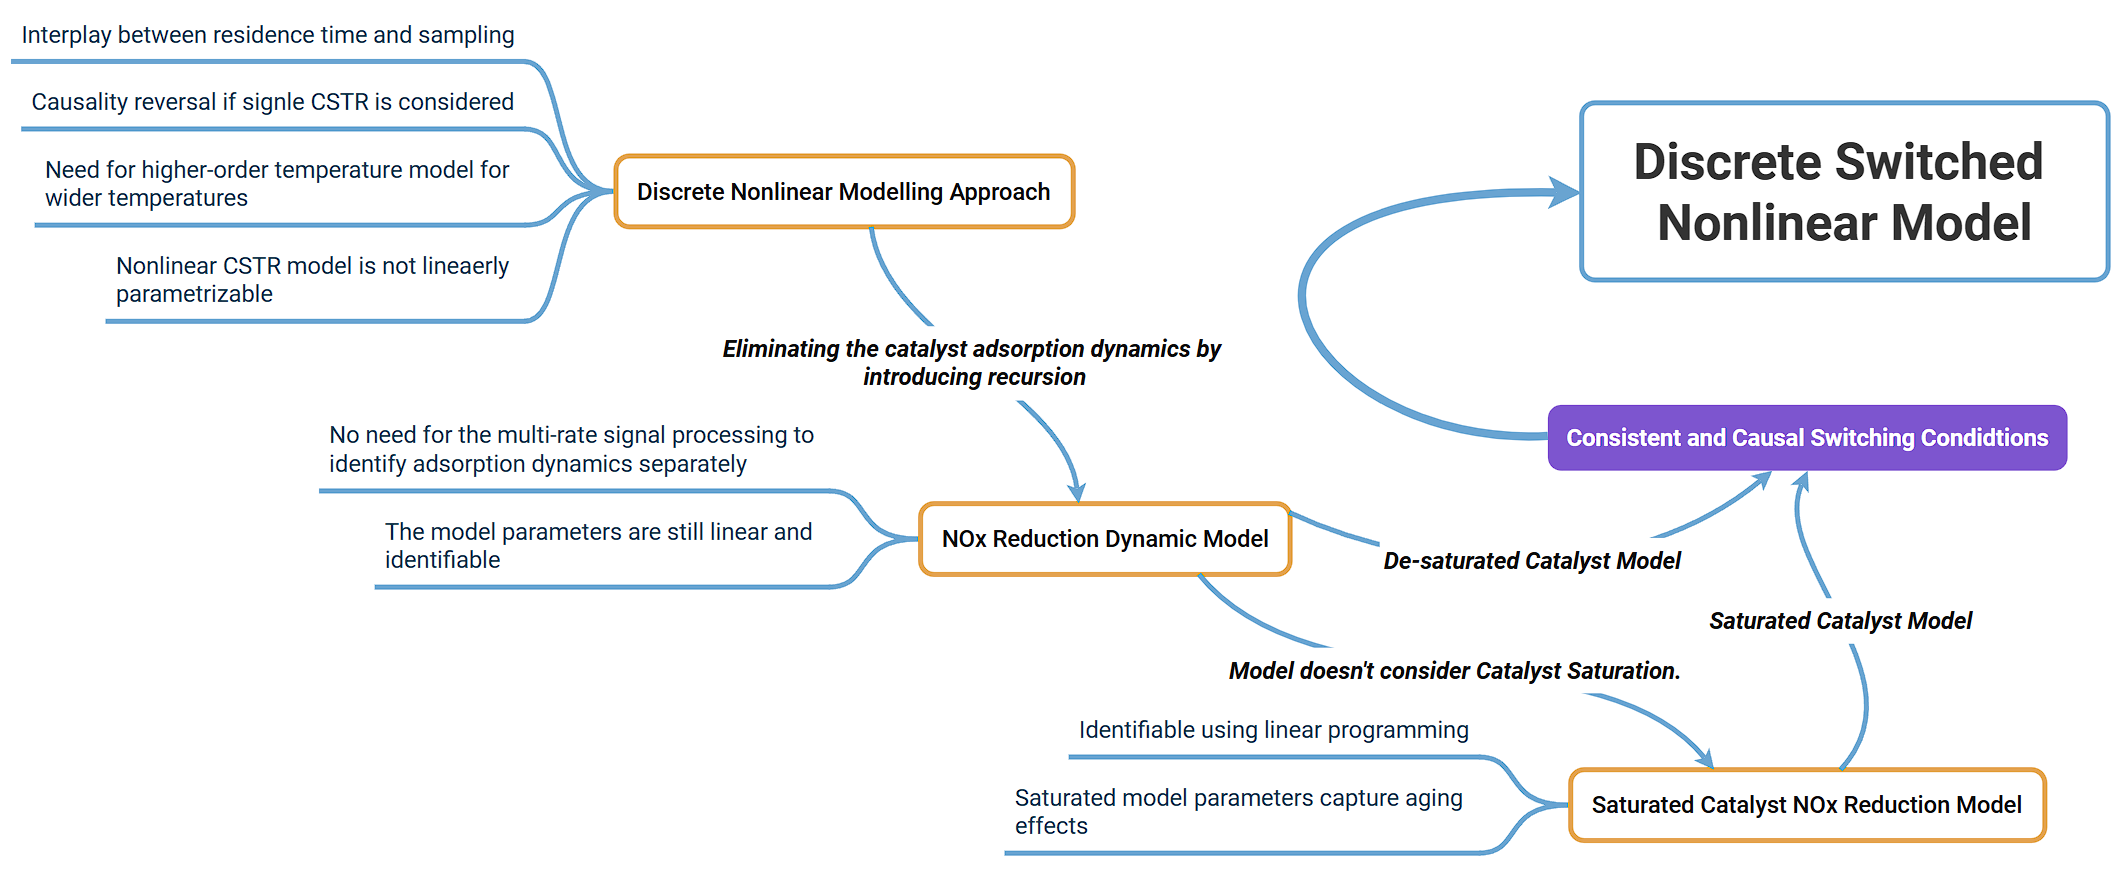
\includegraphics[width = 0.9\textwidth]{\froot/figs/n_figs/problems_soved.png}
        \caption{A map of the developments}
\end{figure}
